\documentclass[border=0.2cm]{standalone}

% Required packages and libraries
\usepackage{circuitikz}
\usetikzlibrary{calc}

\begin{document}
	
	
	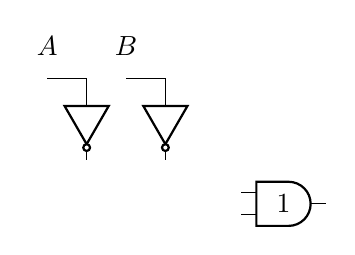
\begin{tikzpicture}
		
	% Circuit style
	\ctikzset{logic ports=ieee,logic ports/scale=0.5}		
			
	\node (A) at (0,0) {$A$};
	\node (B) at (1,0) {$B$};		
	\node[not port, rotate=-90] at ($(A)+(0.5,-1)$) (NotA) {};
	\node[not port, rotate=-90] at ($(B)+(0.5,-1)$) (NotB) {};
		
	\foreach \i in {A,B}{
		\path (\i) -- coordinate (punt\i) (\i |- Not\i.in);
		\draw (punt\i) -| (Not\i.in);
		}
	\node[and port] at ($(B)+(2,-2)$) (gate1) {1};
	
	
	\end{tikzpicture}
	
	
\end{document}